%=========================================================================
% Start of activity on simple harmonic motion.
%=========================================================================
\preClass{Derivatives of Basic Trigonometric Functions}

\begin{problem}
\item Determine the derivatives of the following functions:
  \begin{subproblem}
  \item $\sin(3t)$
    \vfill
  \item $\cos(8t)$
    \vfill
  \end{subproblem}
\item Determine the anti-derivatives of the following functions:
  \begin{subproblem}
  \item $\cos(3t)$
    \vfill
  \item $\sin(8t)$
    \vfill
  \end{subproblem}
\end{problem}


\actTitle{Anti-Derivatives of Trigonometric Functions}
\begin{problem}
\item An object has an acceleration given by
  \begin{eqnarray*}
    a(t) & = & 2\sin(5t) + 5e^{-2t},
  \end{eqnarray*}
  and the initial velocity is $v_0$, and the initial position is $x_0$.
  \begin{subproblem}
  \item Determine the position at any time.
    \vfill
  \item Describe the qualitative behaviour of the position. Does the position
    oscillate, grow, or decay? For what values of $v_0$ and $x_0$ do
    you see different behaviours?
    \vfill
  \end{subproblem}

  \clearpage

\item Determine the first and second derivatives of the following functions.
  \begin{subproblem}
  \item $8\sin(5t)$
    \vfill
  \item $23\cos(2t)$
    \vfill
  \item $8\sin(5t)+2\cos(5t)$
    \vfill
  \item $23\cos(2t)-14\sin(2t)$
    \vfill
  \end{subproblem}

\end{problem}

\actTitle{Simple Harmonic Motion}
\begin{problem}
\item An object is attached to a rigid spring on a horizontal
  table. The origin is determined to be the equilibrium position for
  the object. The mass of the object is 3kg. The object is drawn back
  0.05m and released from rest. The spring obeys Hooke's law with a
  constant, $k=0.4$N/m.
  \begin{subproblem}
    \item Make a sketch of the physical situation.
      \vfill
    \item Make a sketch of the free body diagram. Ignore any friction
      assuming that the friction is negligible for now.
      \vfill
    \item Describe the qualitative behaviour that you expect to see
      from the physical system. How should it behave?
      \vfill
    \item Determine the equation of motion ignoring friction.
      \vfill

      \clearpage

    \item Based on your description of the expected behaviour what
      kind of function mimics that behaviour?
      \vspace{3em}

    \item Assume that the solution has the form
      \begin{eqnarray*}
        x(t) & = & A \sin(\omega t) + B \cos(\omega t),
      \end{eqnarray*}
      where $A$, $B$, and $\omega$ are constants. 
      \sideNote{It is not uncommon to just make a guess at a general
        form, and then check to see if your intuition is consistent
        with the equation.}
      \begin{subproblem}
      \item Determine the velocity and acceleration based on the
        position above.  
        \vfill
      \item Substitute these results into your equation for the motion
        of the object.
        \vfill
        \clearpage
      \item Put all of the sines on one side of the equality and all
        of the cosines on the other side of the equality. What must be
        true about the left and right hand sides?
        \sideNote{Hint: It has to be true for \textbf{all} time!}
        \vspace{6em}
      \item Is it possible to determine values for the constants to
        satisfy the equation and the initial conditions? If so what
        are they?
        \sideNote{Hint: Yes.}
        \vfill
      \end{subproblem}

  \end{subproblem}
\end{problem}

\postClass

\begin{problem}
\item Briefly state two ideas from today's class.
  \begin{itemize}
  \item 
  \item 
  \end{itemize}
\item 
  \begin{subproblem}
    \item
  \end{subproblem}
\end{problem}

%=========================================================================
% Start of activity on finding optimal values of a parameter in SHM
%=========================================================================
\preClass{Simple Harmonic Motion}

\begin{problem}
\item Determine the solution to the following differential equations.
  \begin{subproblem}
  \item $x'' + 4 x  =  0$, $x(0)=0$, $v(0)=1$.
    \vfill
  \item $x'' + 8 x  =  0$, $x(0)=1$, $v(0)=0$.
    \vfill
  \end{subproblem}
\end{problem}


\actTitle{Optimization For Simple Harmonic Motion - Determining The System}
\begin{problem}
\item A spring mass system is to be constructed. The system will be
  assembled on a horizontal table, and friction is ignored. 
  \begin{subproblem}
    \item Make a sketch of the physical situation.
      \vfill
    \item Make a sketch of the free body diagram. Ignore any friction
      assuming that the friction is negligible for now. Assume that
      the spring constant is $k$ N/m and the mass is $m$ kg.
      \vfill
    \item Describe the qualitative behaviour that you expect to see
      from the physical system. How should it behave?
      \vfill
    \item Determine the equation of motion ignoring friction.
      \vfill
  \end{subproblem}

  \clearpage

\item We wish to find values of $k$ and $m$ so that the system reaches
  its maximum distance away from the origin the first time in 0.1
  seconds. Assume that the object is pulled 0.3 m from equilibrium and
  released from rest. What does this imply about the relationship
  between $k$ and $m$?
  \vfill

  \clearpage

\item The cost of the spring depends on $k$ and is $2k^2$\$. The cost
  of the object depends on its mass and is $10m$\$. What is the total
  cost of building the system?

  \vfill

\item Formally express the cost and objective functions:
    \begin{eqnarray*}
      \mathrm{Minimize:} & &  \\
      \mathrm{Constraint:} & & 
    \end{eqnarray*}



\end{problem}

\actTitle{Analysis For Optimization for Simple Harmonic Motion}
\begin{problem}
\item Rewrite the system from the previous set of activities.
    \begin{eqnarray*}
      \mathrm{Minimize:} & &  \\
      \mathrm{Constraint:} & & 
    \end{eqnarray*}

\item Make a sketch of the constraint.
  \sideNote{ Be sure to label your axes and label all important points
    on your graph.}

  \vfill

\item Make a sketch of the cost for various values of the cost. What
  is the general pattern? What do you predict the optimal values of
  $k$ and $m$ will be?

  \vspace{3em}

\clearpage

\item Rewrite the system from the previous set of activities.
    \begin{eqnarray*}
      \mathrm{Minimize:} & &  \\
      \mathrm{Constraint:} & & 
    \end{eqnarray*}

\item Determine analytically the optimal values of $k$ and $m$.
  \vfill


\end{problem}

\postClass

\begin{problem}
\item Briefly state two ideas from today's class.
  \begin{itemize}
  \item 
  \item 
  \end{itemize}
\item 
  \begin{subproblem}
    \item
  \end{subproblem}
\end{problem}

%=========================================================================
% Start of activities on systems of equations
%=========================================================================
\preClass{Systems of Equations}

\begin{problem}
\item Determine the values of $x$ and $y$ that satisfy both of the
  following equations:
  \begin{eqnarray*}
    x + 4y & = & 7, \\
    x + 3y & = & 5.
  \end{eqnarray*}
\end{problem}


\actTitle{Graphical View of Systems of Equations}
\begin{problem}
\item We will graphically determine the values of $x$ and $y$ that
  satisfy both of the following equations:
  \begin{eqnarray*}
    x + 4y & = & 7, \\
    x + 3y & = & 5.
  \end{eqnarray*}
  \begin{subproblem}
  \item Draw a set of axes where $-3\leq x \leq 3$ and $-3 \leq y \leq
    3$. 

    \sideNote{ Be sure to label your axes and label all important
      points on your graph.}

    \vfill

  \item Make a sketch of the relationship $x+4y=7$ on the axes.
  \item Make a sketch of the relationship $x+3y=5$ on the axes.
  \item Circle and estimate the point where both relationships are
    satisfied.
  \end{subproblem}

  \clearpage

\item We will graphically determine the values of $x$ and $y$ that
  satisfy both of the following equations:
  \begin{eqnarray*}
    x^2 + y  & = & 0, \\
    x - 2y^2 & = & 1.
  \end{eqnarray*}

  \begin{subproblem}
  \item Draw a set of axes where $-3\leq x \leq 3$ and $-3 \leq y \leq
    3$. 

    \sideNote{ Be sure to label your axes and label all important
      points on your graph.}

    \vfill

  \item Make a sketch of the relationship $x^2+y=0$ on the axes.
  \item Make a sketch of the relationship $x-2y^2=1$ on the axes.
  \item Circle and estimate the point where both relationships are
    satisfied.
  \end{subproblem}


\end{problem}

\actTitle{Determining Solutions to Systems Analytically}
\begin{problem}
\item Use matrices to determine the values of $x$ and $y$ that satisfy
  both of the following equations:
  \begin{eqnarray*}
    x + 4y & = & 7, \\
    x + 3y & = & 5.
  \end{eqnarray*}

  \vfill

  \clearpage

\item Use matrices to determine the values of $x$ and $y$ that satisfy
  both of the following equations:
  \begin{eqnarray*}
     -x +  y + 5z & = & -13, \\
    -2x +  y + 4z & = & -15, \\
     2x - 2y - 7z & = & 20.
  \end{eqnarray*}

  \vfill

  \clearpage

\item An estimate for the value of $x$ that satisfies $0=3x^2-4$.
  \begin{subproblem}
  \item Draw a set of axes where $-2\leq x \leq 2$. 

    \sideNote{ Be sure to label your axes and label all important
      points on your graph.}

    \vfill

  \item Make a sketch of the relationship $y=3x^2-4$ on the axes.
  \item Make a rough estimate of the value of $x$ where the graph is zero.
    \clearpage

  \item Make a sketch of the tangent line to the graph of the curve
    at your estimate for $x$. Mark the point where the height of the
    tangent line is zero. Is that a better or worse approximation for
    the value of $x$?
    \vspace{2em}

  \item Determine analytically the tangent line to the graph of the curve
    at your estimate for $x$. Determine where the height of the
    tangent line is zero. 

    \vfill

  \item How can you determine if the new $x$ is a better estimate if
    you do not know the true value?

  \end{subproblem}

\end{problem}


\postClass

\begin{problem}
\item Briefly state two ideas from today's class.
  \begin{itemize}
  \item 
  \item 
  \end{itemize}
\item 
  \begin{subproblem}
    \item
  \end{subproblem}
\end{problem}

%=========================================================================
% Start of activity on riemann sums and moment of intertia
%=========================================================================
\preClass{Moment of Inertia}

\begin{problem}
\item A point mass of 2 kg is located at $3\vec{i} + 2\vec{j}$, and a
  point mass of 4 kg is located at $-\vec{i}+3\vec{j}$. Determine the
  moment of inertia around the $x$-axis as well as the moment of
  inertia around the $y$-axis  of the system.

  \vfill

\end{problem}


\actTitle{Moment of Inertia For Discrete Masses}
\begin{problem}
\item A set of point ten masses is lined up on the $x$ axis. They are
  positioned at $x_n=n\cdot 0.1$. The mass of each point mass is
  $\frac{n}{2}$ kg.
  \begin{subproblem}
    \item Make a rough sketch of the system.
      \vfill
    \item Determine the center of mass of the system.
      \vfill
    \item Determine the moment of inertia of the system around the
      $y$-axis.
      \vfill
  \end{subproblem}

  \clearpage

\item A set of point twenty masses is lined up on the $x$ axis. They are
  positioned at $x_n=n\cdot 0.05$. The mass of each point mass is
  $\frac{n}{4}$ kg.
  \begin{subproblem}
    \item Make a rough sketch of the system.
      \vfill
    \item Determine the center of mass of the system.
      \vfill
    \item Determine the moment of inertia of the system around the
      $y$-axis.
      \vfill
  \end{subproblem}

\end{problem}

\actTitle{Moment of Inertia for Continuous Masses}
\begin{problem}
\item A thin metal rod is located on the $x$-axis. The left side of
  the rod is located at $x=0$m and the right hand side is located at
  $x=1$m. The density of the rod is given by $\rho(x)=5x$ kg/m.
  \begin{subproblem}
    \item Make a rough sketch of the system.
      \vfill
    \item Divide it up into $n$ equal sized small segments. Determine
      the location of the left hand side of each small segment.
      \vfill
    \item Determine an approximation for the density of each small
      segment.
      \vfill
    \item Determine the approximate mass and the moment of inertia for
      each small segment.  
      \vfill

      \clearpage

    \item Determine the sum that can be used to approximate the center
      of mass and the sum that can be used to approximate the moment
      of inertia.

      \vspace{5em}

    \item Determine the center of mass and the moment of inertia for
      the rod.

      \vfill

  \end{subproblem}
\end{problem}

\postClass

\begin{problem}
\item Briefly state two ideas from today's class.
  \begin{itemize}
  \item 
  \item 
  \end{itemize}
\item Relate the sum for the center of mass with the integral. Make a
  plot and discuss the relationship with the sum with the area under a
  function. (Which function are you finding the area under?)

  \vfill
\end{problem}


%=========================================================================
% Start of day on moment of inertia and angular momentum.
%=========================================================================
\preClass{Constant Angular Velocity}

\begin{problem}
\item An object moves around a circle with a constant angular
  velocity, $\omega$, and a constant distance from the origin,
  $r$.. The initial angle, $\theta$, is zero.
  \begin{subproblem}
  \item Determine the angle at any time.
    \vfill
  \item Determine the position at any time.
    \sideNote{Use proper vector notation.}
    \vfill
  \item Determine the derivative of the position at any time.
    \vfill
  \item What is the magnitude of the velocity vector?
    \vfill
  \end{subproblem}
\end{problem}


\actTitle{Energy Associated With Constant Angular Velocity}
\begin{problem}
\item An object moves around a circle of radius $r$  at a constant
  rate, $\theta=\omega t$. Its position at any time is $\vec{r}$.

  \begin{subproblem}
    \sideNote{Draw the vector $\delta\vec{r}$ in the plot.}
  \item Use the plot below to graphically represent the difference in
    the positions between any times, $\vec{r}(t+\delta
    t)-\vec{r}(t)$. \\
    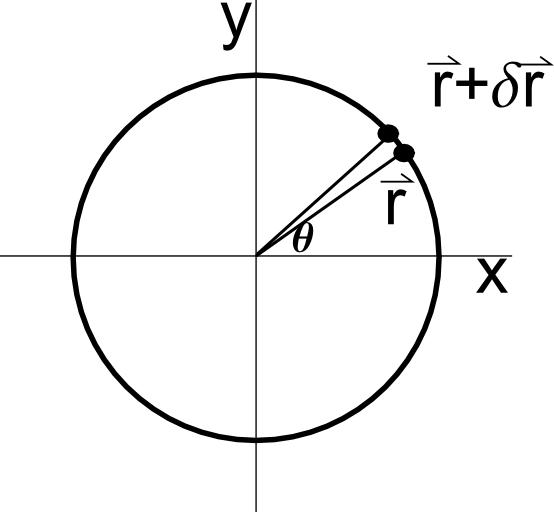
\includegraphics[width=7cm]{ink/week12/circularAcceleration}

    \sideNote{Draw the velocity vectors and then sketch the difference.}
  \item Graphically represent the difference in the velocity vectors,
    $\vec{v}(t+\delta t)-\vec{v}(t)$, at the two positions in the plot below. \\
    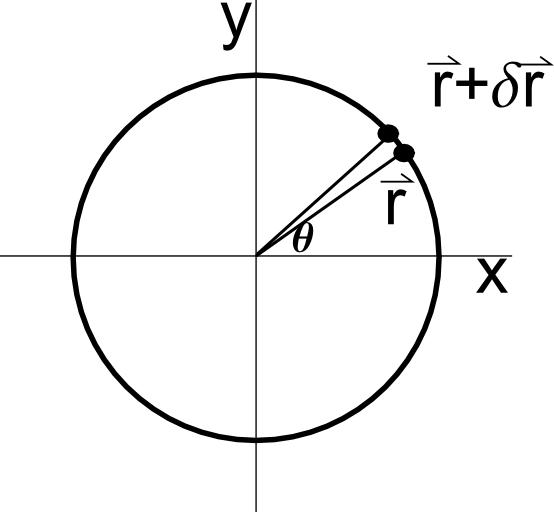
\includegraphics[width=7cm]{ink/week12/circularAcceleration}
    \clearpage
  \item Determine the position at any time. Express the position as
    a vector.\\
    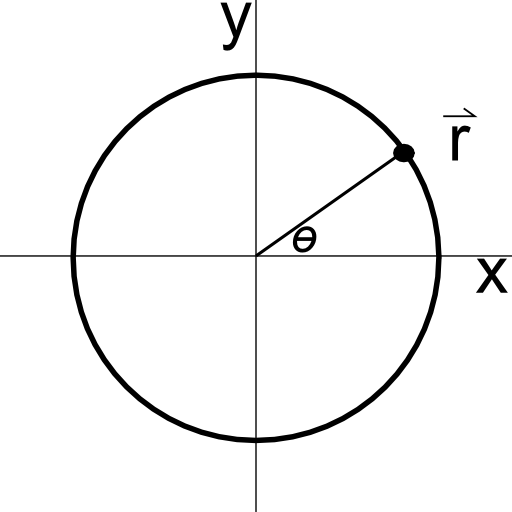
\includegraphics[width=7cm]{ink/week12/circularMotion}
    \vfill
  \item Determine the velocity and the acceleration by taking the
    derivatives of the position with respect to time.
    \vfill
  \item Using the velocity vector determine the energy of the object
    at any time.
    \vfill
  \end{subproblem}
\end{problem}

\actTitle{Angular Velocity}
\begin{problem}
\end{problem}

\postClass

\begin{problem}
\item Briefly state two ideas from today's class.
  \begin{itemize}
  \item 
  \item 
  \end{itemize}
\item 
  \begin{subproblem}
    \item
  \end{subproblem}
\end{problem}





%%% Local Variables:
%%% mode: latex
%%% TeX-master: "labManual"
%%% End:
